\section{Architecture}
\label{section:inflex:arch}

This section describes INFLEX, an architecture which provides edge domains with greater end-to-end resilience.
Rather than probing paths through active or passive means, the network delegates the responsibility for fault detection to end-hosts.
The system relies on packet marking at the host to select a path through the local domain.
This provides far greater scalability in terms of the proportion of traffic and destinations which can be covered, at the cost of requiring small changes to the end-host \ac{TCP}/\ac{IP} stack.
INFLEX is therefore particularly suited for managed environments, such as datacenters or enterprise networks, which not only have greater control over the end-host operating system, but also generate large volumes of traffic towards destinations which cannot be readily upgraded.

An overview of the proposed architecture as applied to a single domain is shown in figure \ref{fig:inflexarch}.
Hosts are connected to the local network through an Openflow-enabled \emph{edge switch}.
While edge switches typically reside within each physical machine, alternative aggregation levels such as the top of rack or end of row may also be used.
Each switch is configured by a specialized controller which resides locally, referred to as an \emph{inflector}.
The local network is configured by a centralized routing controller to provide multiple \emph{virtual routing planes}.
While these planes are necessarily intradomain in scope, some degree of interdomain diversity can also be achieved by changing egress node.

The core of the architecture relies on repurposing the \ac{DS} field in each \ac{IP} packet to provide an in-band signalling channel between the end-host and the inflector.
The header on inbound traffic is set by the edge switch and read by the host, and is used by the inflector to signal which plane a flow has been assigned to.
The header on outbound traffic is set by the host and read by the edge switch, and is used by the transport protocol to ensure that all traffic for the flow is forwarded along the given plane.
Hosts can request a new plane to be assigned by the inflector in case of an end-to-end path fault; this provides efficient cross-layer failure recovery.
The \ac{DS} standard \cite{Blake:1998p370} reserves a pool of code points for local use identified by setting the right-most bit, henceforth referred to as the INFLEX $flag$.
When set, the rest of the \ac{DS} field should be interpreted as containing two fields, shown in figure \ref{fig:inflexarch}. 
An \ac{INF} $label$, which determines the plane over which a packet is forwarded, and an $echo$ bit, which explicitly signals a request from the host or a reply from the network.
The remainder of the description of INFLEX is split across its main components: the end-hosts, the edge switch and the inflector.

\begin{figure}
    \begin{subfigure}[b]{1.0\linewidth}
    \centering
    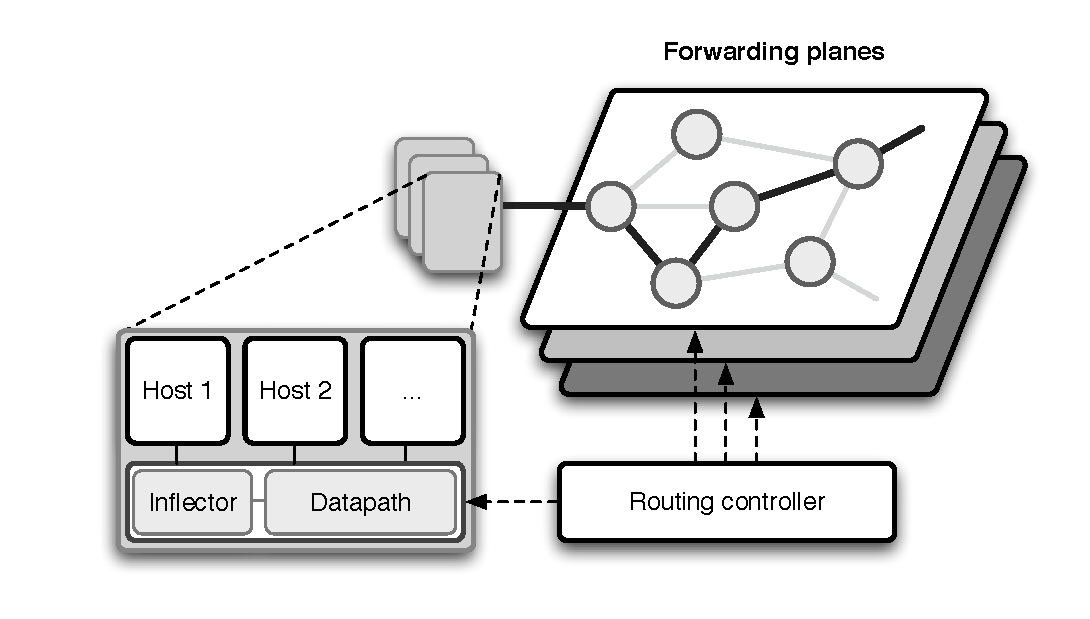
\includegraphics[width=0.7\linewidth]{figures/inflex/arch}
    %\caption{\label{fig:inflexarch}}
    \end{subfigure}
    \begin{subfigure}[b]{1.0\linewidth}
    \centering
    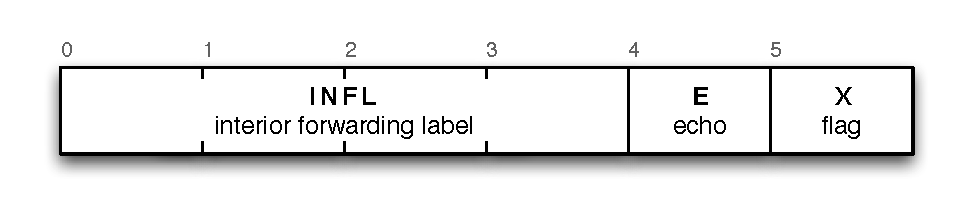
\includegraphics[width=0.5\linewidth]{figures/inflex/header}
    %\caption{\label{fig:inflexheader}}
    \end{subfigure}
    \caption[INFLEX architecture and header.]{INFLEX architecture (above) and header (below). The edge switch forwards traffic across virtual planes set up by a centralized routing service.
    \label{fig:inflexarch}}
\end{figure}

\subsection{INFLEX end-hosts}
\label{section:inflex:host}

INFLEX hosts set the \ac{INF} label of outbound packets according to the value assigned by the inflector, reproducing the path re-feedback design pattern introduced in chapter \ref{chapter:preflex}.
INFLEX however cannot rely on marking by the remote endpoint to trigger network action, as this has been shown to be essentially undeployable.
Instead, path requests are initiated by the sender, which must then await for a network reply piggybacked on a returning packet.

The changes required to support this at the sender side network stack are minimal, and are illustrated in figure \ref{fig:stack}.
Every transport connection occurs over a socket, a local structure containing the variables associated to the ongoing flow.
At the network layer, the local socket has a \ac{DS} value which is copied to every outbound packet (point 1).
Within INFLEX, the transport protocol can trigger a request (point 2), which leads to a network response contained in incoming packets (point 3).

Assume a transport protocol wishes to switch the plane it is currently assigned.
With INFLEX, it can send an \emph{inflection request} by setting the $echo$ bit of the local \ac{DS} field (point 2, figure \ref{fig:stack}).
All subsequent outbound packets will be marked with the resulting value.
The network layer then proceeds to inspect inbound packets, waiting for a network response, as delineated in figure \ref{fig:tcpcode}.
After demuxing an incoming packet, $pkt$, to the corresponding socket, $sock$, a receiver first verifies whether the INFLEX flag is set on the incoming packet (line 2), establishing whether the underlying network supports INFLEX for the given connection.
The receiver must then decide whether it should change the virtual plane the socket is currently assigned.
This can only happen under two conditions.
Firstly, if the \ac{DS} value for the current socket does not have the INFLEX flag set (line 3).
This typically occurs on flow start, where a connection is spawned with a default \ac{DS} value.
Secondly, if the local \ac{DS} value has the echo bit set, there is a \emph{pending} inflection request.
If the incoming packet has the same bit set, it corresponds to the network \emph{reply} (line 4).
Under both previous cases, the connection switches forwarding plane by copy the interior forwarding label from the incoming packet to the local socket, and setting the INFLEX flag (lines 5-6).
These changes are all applied at the \ac{IP} layer -- transport protocols need only to decide when to send inflection requests -- while applications can remain unchanged.

\begin{figure}
    \begin{subfigure}[b]{0.4\linewidth}
        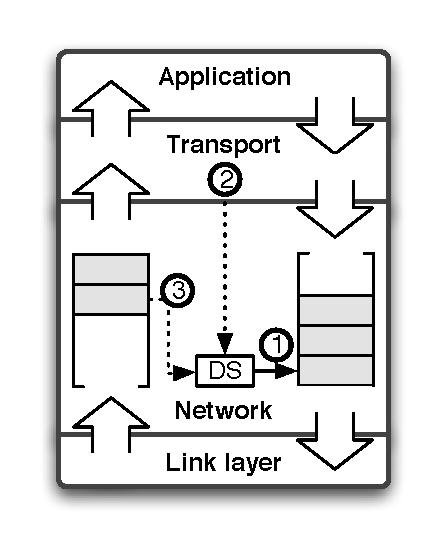
\includegraphics[width=0.9\linewidth]{figures/inflex/stack}
        \caption{\label{fig:stack}}
    \end{subfigure}%
    \begin{subfigure}[b]{0.6\linewidth}
        \vspace*{1.0in}
        \lstset{
        language=C,                % choose the language of the code
        basicstyle=\footnotesize\ttfamily,
        numbers=left,                   % where to put the line-numbers
        stepnumber=1,                   % the step between two line-numbers.
        numbersep=5pt,                  % how far the line-numbers are from the code
        %  backgroundcolor=\color{white},  % choose the background color. You must add \usepackage{color}
        showspaces=false,               % show spaces adding particular underscores
        numberstyle=\scriptsize,
        showstringspaces=false,         % underline spaces within strings
        showtabs=false,                 % show tabs within strings adding particular underscores
        tabsize=2,                      % sets default tabsize to 2 spaces
        captionpos=n,                   % sets the caption-position to bottom
        breaklines=true,                % sets automatic line breaking
        breakatwhitespace=true,         % sets if automatic breaks should only happen at whitespace
        title=\lstname,                 % show the filename of files included with \lstinputlisting;
        }
        \lstinputlisting{\locfolder/tcpapi.c}
        \caption{\label{fig:tcpcode}}
    \end{subfigure}
    \caption[INFLEX host modifications.]{INFLEX (\subref{fig:stack}) host stack and (\subref{fig:tcpcode}) pseudo-code for packet reception.}
\end{figure}

% inflection request
\subsection{The edge switch}

% what is it
The edge switch is primarily responsible for mapping INFLEX marked packets to the appropriate forwarding plane.
On start up its datapath is configured by the local \emph{inflector}, which installs the appropriate flow entries on it in order to construct the processing pipeline in figure \ref{fig:pipeline}.
This pipeline can be partitioned into three distinct blocks, responsible for \emph{triaging}, \emph{policing} and \emph{inflecting} packets.
For clarity, the processing pipeline is conceptually described as a sequence of flow matches across distinct tables.
In practice, an implementer is free to collapse flow tables and entries to improve performance.
An important safeguard is that a legacy pipeline must be present, establishing a default forwarding plane expected to be used by traffic to which INFLEX is not applicable.

\begin{figure}
    \centering
    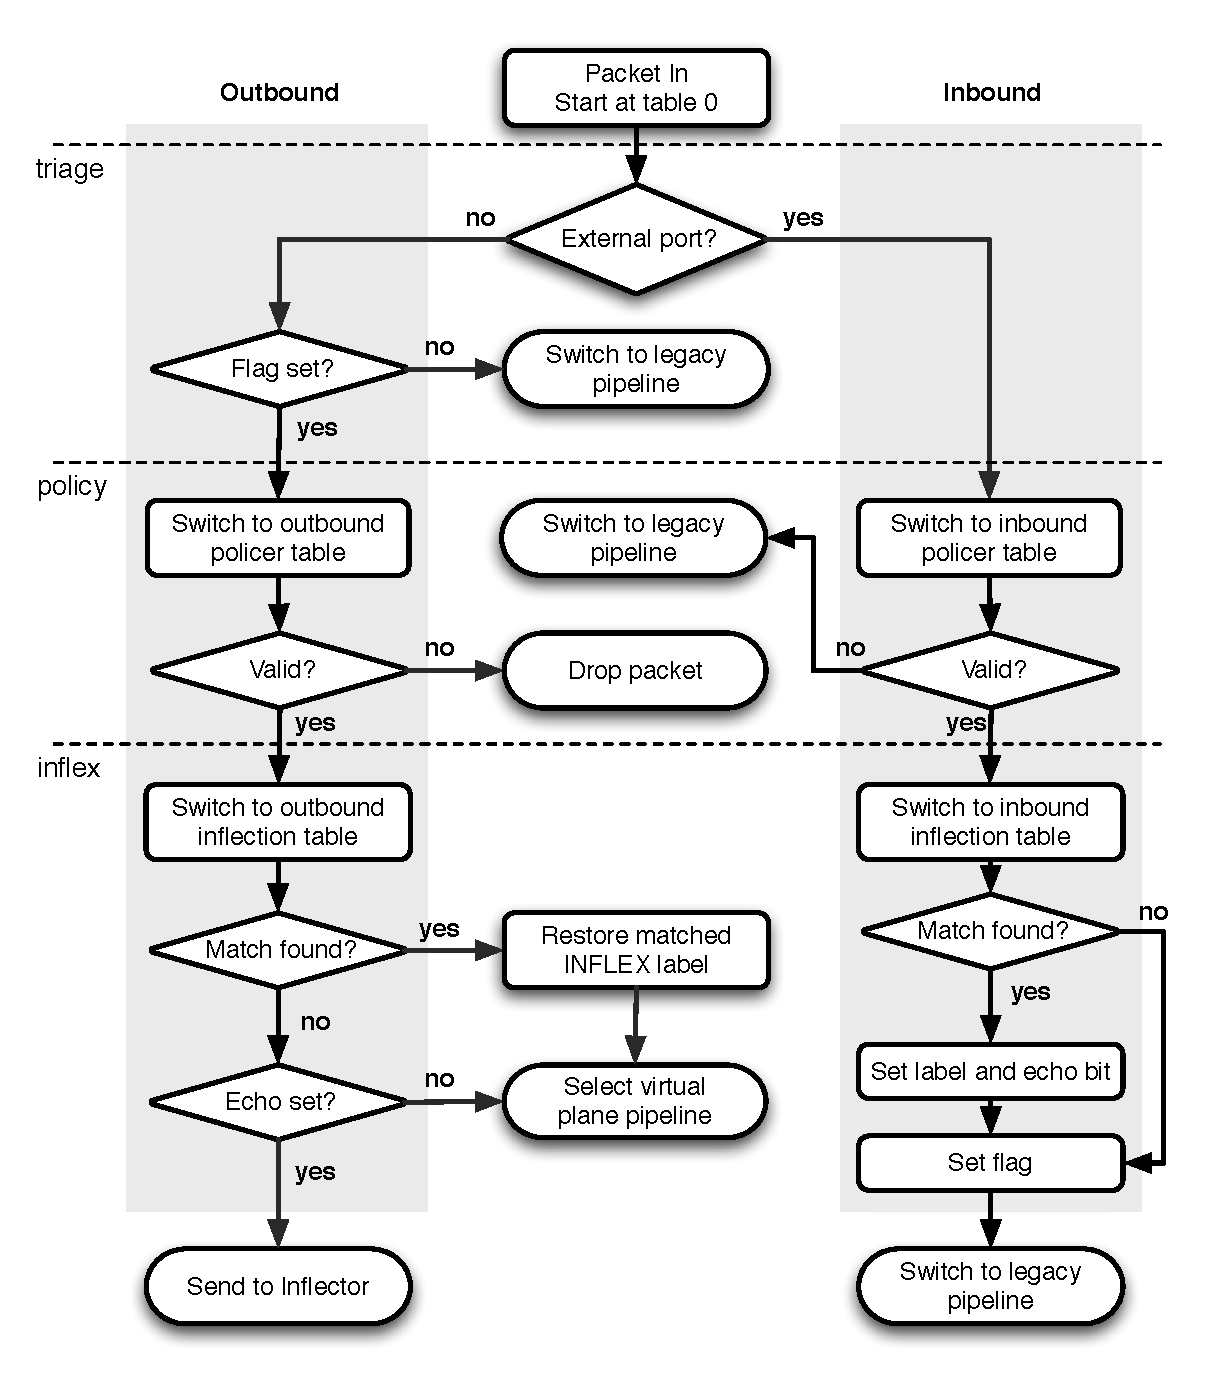
\includegraphics[width=3.5in]{figures/inflex/flowchart}
    \caption{Pipeline installed to the edge switch datapath.}
    \label{fig:pipeline}
\end{figure}

The \emph{triage} phase is responsible for distinguishing whether a packet is \emph{capable} of using INFLEX.
Firstly, INFLEX is only applicable to \ac{IP} packets.
Traffic is then differentiated according to the port on which the packet arrived: if connected to a host, the interface is said to be \emph{internal}, otherwise it is \emph{external}.
Any inbound \ac{IP} traffic may potentially be INFLEX capable and as such can proceed to the next stage.
For outbound \ac{IP} traffic, only packets with the INFLEX flag set require further processing.
Packets for which this flag is not set are assumed to be legacy traffic.

The \emph{policy} phase decides whether a packet is \emph{permitted} to use INFLEX.
For either direction, a packet is compared against a policer table, which contains a set of rules describing local policy concerning INFLEX usage.
The rules applied to each direction however may differ, particularly since outbound packets can be further scrutinized according to the INF $label$.
For example, this allows the outbound policer to enforce which virtual planes are available to specific tenants or applications.
For this reason, the action applied if a packet is matched within the policer table also differs according to direction.
For inbound traffic, a matching rule indicates that the packet does not satisfy local requirements for INFLEX use, and is consequently treated as legacy traffic.
For outbound traffic, a packet is already marked as being INFLEX capable.
Any matching entry therefore indicates that it is in violation of local policy and should consequently be dropped.

Finally, the \emph{inflex} phase processes the respective header and forwards the packet.
A packet is first matched against an \emph{inflection} table in either direction.
This table is detailed in the next section, and can be assumed to contain no matching entry initially.
For outbound traffic, the packet is typically redirected to the  plane mapped by the interior forwarding label.
The one exception are inflection requests, which are forwarded to the local inflector for further processing.
For inbound traffic, the INFLEX flag is marked in order to notify hosts that the flow is INFLEX capable, and the packet is then processed according to the legacy pipeline.

\subsection{The inflector}

% XXX
Each edge switch is controlled by an inflector, an \ac{SDN} controller expected to reside locally.
An inflector is firstly responsible for configuring the underlying datapath according to the previously described pipeline.
Secondly, an inflector must process inflection requests.

Inflection requests require network intervention in assigning a packet to a forwarding plane.
The dynamic nature of this decision process cannot readily be instantiated as a set of static rules at the edge switch, since a same flow must be able to be reassigned to a different plane in case of path faults.
Therefore, inflection requests intercepted at the edge switch must be sent to a controller for further processing.
Rather than overloading a centralized controller however, this decision can be taken locally -- since the inflector manages the local rules associated to each virtual network, it already has full knowledge of the routing table associated to each plane.
Upon receiving such a request, the inflector proceeds in three steps.
It first verifies which virtual networks maintain a valid route for the given destination address.
Given this list of potential planes, it then inspects local policy to verify which planes the packet is allowed to use.
The intercepted packet contains the plane which the flow is currently using -- this plane should be excluded from the candidate list unless there is no other option available.
Finally, a single plane, identified by an interior forwarding label, is selected from the resulting list of candidates.
The selection algorithm is not prescribed by the INFLEX specification, but a reasonable baseline is to select a routing entry proportionally to the assigned route weight.

Having selected an appropriate plane, the inflector installs forwarding rules into either \emph{inflection table}.
In the inbound direction, all packets matching the reverse flow are set to be marked with the corresponding \ac{INF} $label$.
This conveys the selected forwarding plane back to the host.
In the outbound direction, all packets matching the flow are to be processed according to the $label$.
This guarantees that any packet sent between the inflection request and its response are forwarded in a consistent manner.
Rules installed to the inflection tables are ephemeral by nature, with a hard timeout of 1 second (the minimum permitted in the Openflow standard).
This enables per-flow granularity with minimum flow state while also rate limiting inflection requests.
Furthermore, flow entries can be configured to be sent to the controller upon expiry.
This potentially allows the inflector to collect realtime information on the availability of each forwarding plane, allowing for further refinement of the plane selection algorithm.
